% Keep these two lines in order for typesetting to work w/ the funny fonts.
%!TEX TS-program = xelatex
%!TEX encoding = UTF-8 Unicode

\documentclass[12pt]{article}
\usepackage[margin=1.25in]{geometry}
\usepackage[config, font=small, labelfont={sf,bf}, textfont=sf]{caption,subfig}
\usepackage{graphicx}
\usepackage{hyperref}
\usepackage{amssymb}
\usepackage{hyperref}
\usepackage{fontspec,xltxtra,xunicode}
\usepackage{setspace}
\defaultfontfeatures{Mapping=tex-text}
%\setromanfont[Mapping=tex-text]{Baskerville}
\setromanfont{Fanwood Text}
%\setsansfont[Scale=MatchLowercase,Mapping=tex-text]{Gill Sans}
%\setsansfont[Scale=MatchLowercase]{Cabin}
%\setmonofont[Scale=MatchLowercase]{Andale Mono}
%\usepackage[margin=10pt,font=sf,labelfont=bf, labelsep=endash]{caption}

%% \usepackage{titlesec}
%% \newfontfamily\sectionfont{League Gothic}
%% \titleformat*{\title}{\Huge\bfseries\sffamily}
%% \titleformat*{\section}{\Huge\bfseries\sffamily}
%% \titleformat*{\subsection}{\Large\bfseries\sffamily}
%% \titleformat*{\subsubsection}{\large\bfseries\sffamily}

\newenvironment{packed_enum}{
\begin{enumerate}
  \setlength{\itemsep}{1pt}
  \setlength{\parskip}{0pt}
  \setlength{\parsep}{0pt}
}{\end{enumerate}}

\title{Dissertation Proposal:\\
Interaction Techniques for Sketch-based Design}
\author{Gabe Johnson}

\begin{document}
\maketitle

\doublespacing % Note: there is also a doublespacing command after the
               % page of figures, since that page changes spacing
               % temporarily.

\begin{abstract}
Rapid prototyping machines like laser cutters and 3D printers are
becoming more common. However, the associated modeling software has a
significant learning challenge for novice users. I propose to create a
modeling system that allows for design of objects via freehand
sketching, a skill that most people already have. Sketch-based
interaction is viewed as a promising design method, but unlike
traditional WIMP applications there are no standard interaction
techniques for sketch-based applications. The proposed system will
explore sketch-based interaction techniques for moderately complex
tasks such as the design of objects for production via laser cutter. I
will develop a series of sketch-based interaction techniques that are
appropriate for their tasks and work well as an ensemble. 
Additionally, I will test the utility of this system against existing
design methods and tools.
\end{abstract}

\section{Problem Statement}

In recent years, computational support for sketching has focused
mostly on the early phases of design. This is for good reason: paper
and pencil sketching remain central to design practice despite the
ubiquity of powerful computer-based design tools. Sketching allows
people to quickly jot down ideas or exchange thoughts with others;
they provide a medium through which designers think about problems and
potential solutions. Freehand drawing is an activity that nearly all
designers---professional and avocational alike---readily employ.

Ideas that begin as rough sketches may eventually be prototyped with
rapid prototyping machinery such as 3D printers, CNC routers, or laser
cutters. Over time, this sort of machinery will become more
affordable, utilize a wider range of materials, and produce
higher-quality output. Rapid fabrication machines offer the potential
to enable people to take active control of the design of their world,
rather than being passive consumers of products somebody else has
made.

However, there remains a gap between the technology used to design and
the technology used to prototype physical items. Today, a typical
design process might involve several paper sketches, followed by a
session with a computer modeling system such as SketchUp, SolidWorks,
or Rhino. When the designer is satisfied with the CAD model, the rapid
fabrication machinery is put to work. The designer can then evaluate
the output and decide what to do next: keep the design as it is,
change the CAD model, or ``go back to the drawing board'' and sketch
new ideas.

This proposal describes an alternate approach that brings the
sketching and computer modeling activities together in the same
tool. It lets users sketch as roughly or precisely as they like,
iteratively and interactively making models that can be manufactured
using rapid fabrication machines. Specifically, the system will
support users to model objects for production on laser cutters. Such
objects are composed of flat, rigid parts. Figure \ref{fig:flat} shows
examples household objects that could be designed using the proposed
system and produced with a laser cutter.

This project's first motivation is to empower those who are not
professional designers to create meaningful objects with rapid
fabrication machines. It can not be assumed that these users have been
taught to draw as an architect would have been, nor can it be assumed
they have invested a great deal of time to learn the often complicated
modeling software that was developed for professional use.

The second motivation is to explore the space of sketch-based
interaction as it applies to modeling physical objects. A success
criterion is that the user should never need (or want) to set down
their stylus in favor of keyboard or mouse input.

\begin{figure}
\centering 
\subfloat[] {
  \label{fig:flat-a} 
  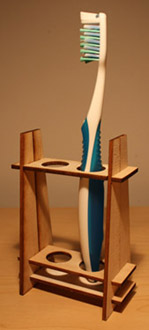
\includegraphics[height=2.2in]{img/flat-a.jpg}
}
\hspace{1cm} \subfloat[] {
    \label{fig:flat-b}
    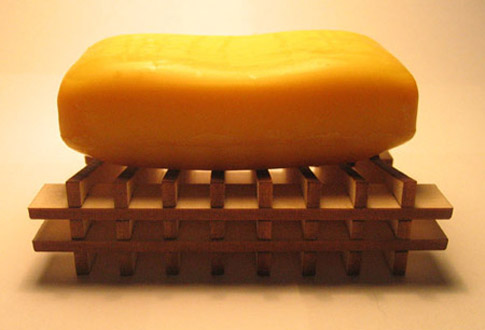
\includegraphics[height=2.2in]{img/flat-b.jpg}
}
\caption{Household objects made with a laser cutter.}
\label{fig:flat}
\end{figure}

\subsection{Conversational Sketch-based Interaction}

The premise of interactive systems is that there is an ongoing
``conversation'' between the user and computer. In sketch-based
systems, users ``speak'' with a stylus; computers ``speak'' with
graphics. Just as humans have social norms for engaging in
conversation that allow us to talk to people we have not met before,
there should norms for human-computer interaction in sketch-based
systems so our experience from one application can be used in the
next.

% Not sure if this para is necessary but I need something to lead in
Olsen~\cite{olsen-ui-research} argues the dominant paradigm of ``one
display, one keyboard, one mouse'' hinders progress in interactive
systems that use alternate hardware configurations. There is no
standard for sketch-based interaction, where typical hardware is a
pen-sensitive display and stylus. In recent years, researchers have
begun to give more attention to interaction aspects of sketch
recognition-based user interfaces, but the extent of this work remains
limited.

For each of the several technical challenges in sketch-based systems
research there is a human component. Segmentation and recognition are
concerned with perceptual and semantic interpretation, which is
inevitably wrong on occasion. When does the system attempt to
recognize input? How detailed must the recognition be in order to
match the user's intentions? What salient aspects are to be
recognized? How does the system tell the user what has been
recognized? When should this occur? How can the user work with the
system to recover from mistakes?

The answer to these questions presumably begins with ``it depends on
what the user is trying to achieve.'' In the proposed system, ideas
are gradually refined from sketches into manufacturable models. The
user's goals are different early in this process compared with latter
stages. Early in this process the user's goal is to simply record
ideas, possibly to share with other people. The early phase is usually
about \textit{big ideas}. Later, the user's goals might be to add
specific details such as lengths, angles, and how different parts
interact---this phase is about \textit{details}.

\subsection{Proposal Organization}

The remainder of the proposal is organized as follows. First I present
a hypothetical motivating scenario that describes how the system might
be used, and relates many of the sketch-based interaction
techniques. Previous related work on sketch recognition, sketch
interaction, and rapid fabrication is then discussed. Next I detail my
own efforts in sketching and design tools for fast fabrication. The
proposal ends with the thesis contributions, a discussion of how the
system will be evaluated, and a time line for project completion.

\section{Motivating Scenario}

\begin{figure}[] 
\centering
\subfloat[Initial sketches of possible designs.] { 
   \label{fig:initial-sketches}
   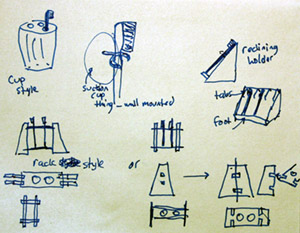
\includegraphics[width=2.0in]{img/physical-sketches.jpg} 
}
\hspace{5mm} \subfloat[Sketch of the user's preferred design in
  greater detail.] {
   \label{fig:final-sketch}
   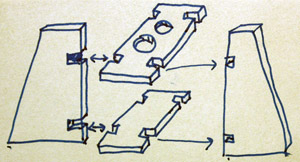
\includegraphics[width=2.0in]{img/final-sketch.jpg} 
}
\hspace{5mm} \subfloat[Final physical output made with a laser
  cutter.] {
   \label{fig:final-physical-output}
   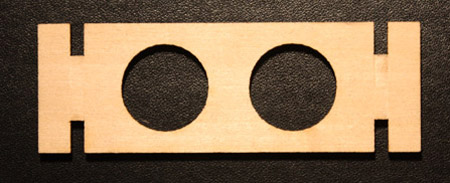
\includegraphics[width=3.0in]{img/final-physical-output.jpg} 
}
\caption{Initial sketches and photograph of one part of the physical
  output.}
\label{fig:physical-sketches}
\end{figure}

This section illustrates how a user might design the toothbrush holder
shown in Figure~\ref{fig:flat-a} using the proposed system. There is
also a video of this process at the URL
\href{http://vimeo.com/17997357}{http://vimeo.com/17997357}.

Some toothbrush holders rest on the sink while others are attached to
the wall in some way; some hold a single toothbrush while others
support up to four; some are similar to cups while others resemble
racks. The user makes a variety of drawings (see
Figure~\ref{fig:initial-sketches}) to help think about particular
needs and preferences, and decides to focus on a rack-style holder,
shown in the lower right corner of the initial sketch. This design
features two slats supported at each end by side pieces. Toothbrushes
fit through holes in the top slat and rest on the solid bottom slat.

So far the user had simply been sketching without leveraging
computation. But now the user is ready to begin thinking about details
of how the object will be made, and the system can let the user supply
information about dimensions.

There are three unique parts used in this design, shown in
Figure~\ref{fig:final-sketch}. To illustrate the interaction
techniques featured in this system, the remainder of this section
focuses on the design of the part with circular holes in it (shown in
~Figure\ref{fig:final-physical-output}). Figures
\ref{fig:ix-draw-bounds}--\ref{fig:ix-draw-guides} depict the design
process.

From the onset of this process the user realizes that toothbrush
holders come in many sizes, and it is not completely apparent what the
``right'' dimensions are. Some properties like width and depth should
be parametric, which allow the model to produce objects in a variety
of sizes. Much of the following activity is guided by the desire to
retain flexibility in the model.

The user begins drawing the part as a rectangle. Even though the user
knows the finished slat will have notches cut from several locations,
it is easy to begin by drawing it as a rectangle and removing the
material for the notches later. The user asks the system to interpret
the drawing, and the system replaces the input with a beautified
rectangle.

The slat features four notches, each of the same size. To make these
the user begins by drawing just one. A pen stroke that begins and ends
outside a part, but traverses a part boundary will remove material
(see Figure~\ref{fig:ix-remove-from-edge}). This cutting gesture has
been used in earlier systems like Teddy~\cite{igarashi-teddy}.

Next the user would like to add dimension details to the
notch. Because the notch is relatively small on the screen, it is
helpful to zoom in (Figure~\ref{fig:ix-zoom-pan}). Zooming is
performed by a double-circle gesture, inspired by the zooming
technique from Lineogrammer~\cite{zeleznik-lineogrammer}. Clockwise
and counter-clockwise gestures zoom in and out respectively. For a few
moments after zooming, a widget appears that lets the user pan to the
desired location.

The user would like to parameterize the notch dimensions so they may be
changed later by name. To parameterize a length, the user draws a line
with arrows on both ends near the desired line segment, and labels it
with writing (Figure~\ref{fig:ix-notch-param}).

The first notch's geometry should be replicated for the next
three. The user can give the system a
\textit{hint}~\cite{mcdaniel-gamut} by selecting existing
elements. The selection is used as a strong suggestion for the next
editing operations. The user selects the notch by tracing over it. The
selection is graphically acknowledged. Next the three more notches are
drawn at the appropriate places. The \textit{nd} and \textit{nw}
parameters are implicitly copied from the original to the other
notches because they were part of the hint (see
Figure~\ref{fig:ix-hints}).

The user proceeds to give names to the height and width lengths. In
addition the width is given a value, expressed in terms of height (see
Figure~\ref{fig:ix-set-params}). This updates the drawing to reflect
the new width as a function of current height.

Designers often use external tools such as straight edges, French
curves, or stencils when precision is desired. Alternately, people
might lightly draw \textit{construction lines} that guide subsequent
drawing activity~\cite{company-sketching-in-engineering}. The user
would like to draw two circles equidistant from the center of the
slat. To precisely indicate the center of the part, the user draws two
construction lines through the midpoints of two sides
(Figure~\ref{fig:ix-guide-lines}). The designer uses these guides
to place ``fat dots'' in several locations.

The user now wonders if three holes might fit, so two additional
circles are made without using guides. The user decides to stick with
the two-hole design, so the two new holes are erased using a
scribble-out gesture (Figure~\ref{fig:ix-erase}). It is inevitable
that the system's interpretations will occasionally conflict with the
user's intentions. Rather than aiming for perfect recognition (which
is impossible due to ambiguity) this system aims to enable users to
easily recover from such recognition conflicts by providing
appropriate interaction techniques.

The user continues to work, using interaction techniques already
described to parameterize the distance between the center of the part,
and the center of the holes. The user also draws one point where one
of the hole boundaries will be (Figure~\ref{fig:ix-combined}).

The user can hide non-boundary elements like parameters and
construction lines and view the drawing (Figure~\ref{fig:ix-final})
before making the part on a laser cutter. Compare this with the final
output shown earlier in Figure~\ref{fig:final-physical-output}.

\newpage
\newgeometry{left=0.75in,right=0.75in,top=1in,bottom=1in}
\twocolumn

\begin{figure}[] 
\centering
\subfloat[] { 
   \label{fig:ix-draw-bounds-1}
   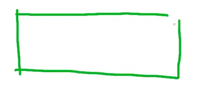
\includegraphics[width=1.35in]{img/ix-draw-bounds-1.png} 
} \subfloat[] {
   \label{fig:ix-draw-bounds-2}
   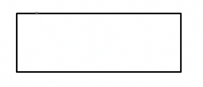
\includegraphics[width=1.35in]{img/ix-draw-bounds-2.png} 
}
\caption{System identifies and rectifies closed shapes.}
\label{fig:ix-draw-bounds}
\end{figure}

\begin{figure}[] 
\centering
\subfloat[] { 
   \label{fig:ix-remove-from-edge-1}
   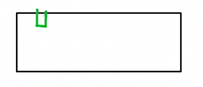
\includegraphics[width=1.35in]{img/ix-remove-from-edge-1.png}
} \subfloat[] {
   \label{fig:ix-remove-from-edge-2}
   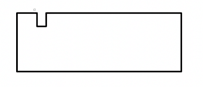
\includegraphics[width=1.35in]{img/ix-remove-from-edge-2.png} 
}
\caption{Remove (or add) material with gestures that cross the part
  boundary.}
\label{fig:ix-remove-from-edge}
\end{figure}

\begin{figure}[] 
\centering
\subfloat[] { 
   \label{fig:ix-zoom-pan-1}
   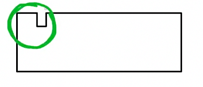
\includegraphics[width=1.35in]{img/ix-zoom-pan-1.png} 
} \subfloat[] {
   \label{fig:ix-zoom-pan-2}
   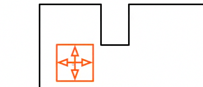
\includegraphics[width=1.35in]{img/ix-zoom-pan-2.png} 
}\\
 \subfloat[] {
   \label{fig:ix-zoom-pan-3}
   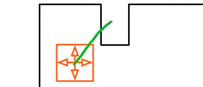
\includegraphics[width=1.35in]{img/ix-zoom-pan-3.png} 
} \subfloat[] {
   \label{fig:ix-zoom-pan-4}
   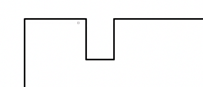
\includegraphics[width=1.35in]{img/ix-zoom-pan-4.png} 
}
\caption{Double-spiral gesture zooms in (clockwise) or out
  (counter-clockwise)~\cite{zeleznik-lineogrammer}. Pan widget appears
  after zoom gesture.}
\label{fig:ix-zoom-pan}
\end{figure}

\begin{figure}[] 
\centering
\subfloat[] { 
   \label{fig:ix-notch-param-1}
   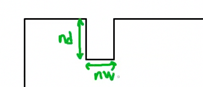
\includegraphics[width=1.35in]{img/ix-notch-param-1.png} 
} \subfloat[] {
   \label{fig:ix-notch-param-2}
   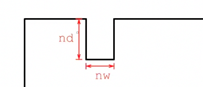
\includegraphics[width=1.35in]{img/ix-notch-param-2.png} 
}
\caption{Make length parameters with double-headed arrows and text.}
\label{fig:ix-notch-param}
\end{figure}

\begin{figure}[] 
\centering
\subfloat[] { 
   \label{fig:ix-hints-1}
   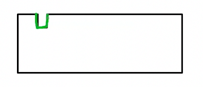
\includegraphics[width=1.35in]{img/ix-hints-1.png} 
} \subfloat[] {
   \label{fig:ix-hints-2}
   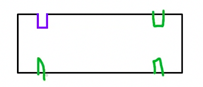
\includegraphics[width=1.35in]{img/ix-hints-2.png} 
}
\caption{Make hints by selecting elements. The hint guides
  interpretation.}
\label{fig:ix-hints}
\end{figure}

\begin{figure}[] 
\centering
\subfloat[] { 
   \label{fig:ix-set-params-1}
   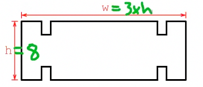
\includegraphics[width=1.35in]{img/ix-set-params-1.png} 
} \subfloat[] {
   \label{fig:ix-set-params-2}
   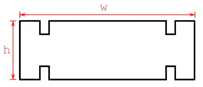
\includegraphics[width=1.35in]{img/ix-set-params-2.png} 
}
\caption{Set parameter values. Model updates to reflect new
  constraints.}
\label{fig:ix-set-params}
\end{figure}

\begin{figure}[] 
\centering
\subfloat[] { 
   \label{fig:ix-guide-lines}
   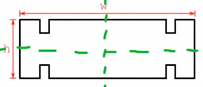
\includegraphics[width=1.35in]{img/ix-guide-lines.png} 
} \subfloat[] {
   \label{fig:ix-guide-dots}
   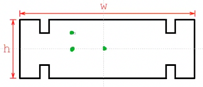
\includegraphics[width=1.35in]{img/ix-guide-dots.png} 
}\\
 \subfloat[] {
   \label{fig:ix-guide-circles}
   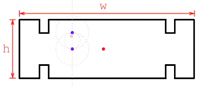
\includegraphics[width=1.35in]{img/ix-guide-circles.png} 
}
\caption{Guides facilitate accurate
  drawing. Guidelines~\subref{fig:ix-guide-lines} and reference
  points~\subref{fig:ix-guide-dots} drawn as indicated; circular
  guides~\subref{fig:ix-guide-circles} made by selecting reference
  points.}
\label{fig:ix-draw-guides}
\end{figure}

\begin{figure}[] 
\centering
\subfloat[] { 
   \label{fig:ix-erase-1}
   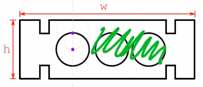
\includegraphics[width=1.35in]{img/ix-erase-1} 
} \subfloat[] {
   \label{fig:ix-erase-2}
   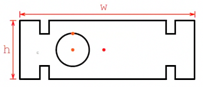
\includegraphics[width=1.35in]{img/ix-erase-2} 
}
\caption{The user draws two holes but changes their mind and erases
  them with a scribble gesture.}
\label{fig:ix-erase}
\end{figure}

\begin{figure}[] 
\centering
\subfloat[] { 
   \label{fig:ix-combined}
   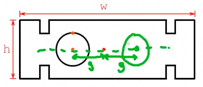
\includegraphics[width=1.35in]{img/ix-combined.png} 
} \subfloat[] {
   \label{fig:ix-final}
   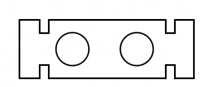
\includegraphics[width=1.35in]{img/ix-final.png} 
}
\caption{Combine techniques to finish part.}
\label{fig:ix-final-steps}
\end{figure}
\restoregeometry
\newpage
\onecolumn
\doublespacing
\section{Related Work}

While ``the design process'' has important differences from domain to
domain, nearly all designers sketch. The ease of freehand drawing
allows people to quickly externalize ideas to analyze their
consequences, as well as to help see new
solutions~\cite{lawson-designers-think,goldschmidt-dialectics}. Many
design professions formalize the importance of sketching by making it
central to the schooling: architects, industrial and interaction
designers, and mechanical engineers are all explicitly taught to
sketch. And even though sketching is not taught in other design
domains (like software engineering), freehand drawing is still
commonly done. Even people that consider themselves non-designers make
quick drawings to help think through everyday problems like how the
furniture in their house might be arranged. Freehand drawing is done
by people of all ages~\cite{goldschmidt-backtalk} and experience
levels~\cite{suwa-analysis-students}.

The prior literature on technical aspects related to this project can
be described in three categories: sketch recognition, calligraphic
interaction, and rapid fabrication.

\subsection{Sketch Recognition}

Ideally, computers would understand sketches as readily as
people. This is of course a very difficult problem of artificial
intelligence. Therefore, researchers often restrict the problem by
obliging users to draw shapes in prescribed
ways~\cite{rubine-recognizer,wobbrock-dollar}, or by limiting the user
to work in specific domains with fairly small visual vocabularies (on
the order of tens of meaningful primitives). Further improvements are
made if the system can correctly identify contextual clues (often
driven by domain semantics) to prune unlikely
interpretations~\cite{gross-ecn-uist,do-phd-thesis}.

Many sketch recognition approaches include at least two distinct
tasks. The first is primitive ink parsing (also known as
segmentation). This process interprets raw user input (time-ordered
point sequences) into atoms such as straight lines, curves,
intersections, and corners \cite{paulson-paleosketch}. In systems that
recognize multi-stroke elements, this step is also usually responsible
for determining which atoms should be considered together. Segmenters
often leverage temporal
data~\cite{sezgin-masters-early-ink,wolin-smr}, spatial
data~\cite{kara-recognizer-cg}, or both~\cite{cates-phd-thesis}.

The second task is to analyze these atoms to perform
recognition. Recognition accuracy is dependent on the quality of the
primitive ink parsing. To increase robustness and accuracy, some
techniques supply multiple possible segmentations to the
recognizer~\cite{alvarado-dynamic-bayes}.

Design sketches from most domains combine diagrammatic ink and written
language. It is helpful for the system to identify what is writing and
what is not~\cite{shilman-discerning-structure}. If done correctly,
such meta-recognition can ease the recognition task by reducing the
amount of input to interpret.

\subsection{Calligraphic Interaction}

Applications often interpret user input differently depending on which
\textit{mode} the program is in (e.g. line mode, circle mode, text
mode, and so forth). This simplifies the computer's task because it is
unambiguous how to interpret user input. But this complicates the
user's task because they must manage modes while designing. 

One way to make mode changing transparent is to infer the user's
intention. The inferred mode protocol~\cite{saund-inferred-mode}
analyzes user input to determine if user input is unambiguous enough
for action to be taken. When ambiguity exists, the system might
mediate by asking what was intended, or take no action and wait for
additional input~\cite{mankoff-burlap}.

Another way of easing the problem of mode is to make it easier for
users to change between them. This might involve buttons pressed with
the non-dominant hand, or with pen gestures such as dwell or pigtail,
or by using pressure\cite{li-mode-switching}.

Drawn gestures can be powerful, but users must first know of their
existence. Some gestures seem easy enough that people do not
necessarily need to ``learn'' them (e.g. scribble over something to
erase it), but many gestures are hard to remember and might be nearly
impossible to discover without assistance. GestureBar is a novel
approach to let users discover and practice
gestures~\cite{bragdon-gesturebar}.

Last, mode can be managed as it is in traditional applications, where
people use on-screen widgets. These widgets may be present at all
times~\cite{forbus-nusketch-battlespace}, invoked via
gesture~\cite{grossman-hover-widgets,kurtenbach-marking-menus} or by
placing the pen near onscreen
ink~\cite{marinkas-shadowbutton,grossman-handle-flag}.

Design sketches often involve a combination of text and pictures. In
situations where the computer should recognize text (or at least
recognize which ink specifies writing) it is necessary to distinguish
between what is text and what is not. One approach is to automatically
classify input as text or non-text based on a statistical analysis of
its visual properties \cite{patel-detect-text}. Another approach is to
ask the user to specify what is text by performing a gesture. This was
the approach taken by the developers of
Lineogrammer~\cite{zeleznik-lineogrammer}.

The proposed work is similar to Lineogrammer and the ParSketch
system~\cite{company-sketching-in-engineering,naya-parsketch} in
several key respects: they both offer the ability to create precise
drawings by using sketch and gesture recognition, and they both eschew
modal input when possible. The proposed work integrates many more
sketch- and pen-based interaction techniques. Also, because it is in
support of machined output, it is necessary that the drawing give
enough detail that objects can be manufactured.

\subsection{Rapid Fabrication}

In the 1980s, inexpensive but high-quality printers enabled desktop
publishing to become common. Prior to this, people relied on printing
companies and graphic designers if they needed to create
professional-looking printed output. 

Physical prototyping machines might very well become as common as
desktop printers, which will change our perception of the role of
computers~\cite{eisenberg-fab}. Home fabrication means people could
make their things, from craft items to replacement parts when things
break. This is a democratizing turn of events, but the current crop of
software for designing these objects is typically too hard for most
people to use~\cite{landay-design-tools} and is a limiting factor.

Sketching has long been a subject of study by makers of physical
things. Leonardo da Vinci's legendary sketchbooks are an early example
of the utility of sketching for both thinking and for
specifying. Demonstrations of the earliest computer-based sketching
system, Sketchpad~\cite{sutherland-sketchpad}, were often focused on
drawing machinable parts.

Until fairly recently, many systems for 3D modeling or fabrication
have used the term ``sketching'' as shorthand for ``quick'' in
comparison to traditional CAD modeling
interfaces~\cite{bloomenthal-sketch-n-make,pugh-thesis-viking,zeleznik-sketch}. Google
SketchUp is a commercial example of this.

Many researchers interested in sketch input for designing physical
objects have been concerned with recognizing 3D drawings,
e.g.~\cite{lipson-correlation,masry-3d-sketch}. Such work focuses on
interpreting the 3D geometric meaning of a finished 2D sketch. In a
sense, that approach assumes that the designer's creative work has
concluded and the job of the computer is to translate the drawing into
a 3D model. This contrasts with interactive approaches that aim to
support an ongoing conversation between the human and computer. A
conversational system tacitly acknowledges that the user's ideas are
not fully formed from the onset, but become progressively clearer as
they work.

With the availability of prototyping machines, sketch-based systems
for fabrication are beginning to receive attention. The Furniture
Factory accepts 2D sketch input that is recognized as a 3D
configuration of planes~\cite{oh-fab}. The user adds pieces
incrementally, so there is no need to make a complete sketch all at
once. The system automatically computes how these planes can be joined
together and generates a series of 2D pieces that to be produced with
a laser cutter.

Saul's Sketch Chair \cite{saul-sketch-chair} is another sketch-based
system for generating furniture. It lets users sketch the contours of
a chair's seat and back rest, and using a different drawing mode, add
legs. The system includes a sophisticated physical simulator to let
the designer explore its physicality (for example to determine if it
will remain upright), and if it will be comfortable. It also allows
designers to change subtle properties of curves using onscreen control
handles.

Plushie lets people make bulbous textile objects such as plush toys or
balloons~\cite{mori-plushie}. Users iteratively design objects by
drawing object boundaries or giving editing commands by sketched
gesture. The interaction is based on prior systems in the Teddy family
tree~\cite{igarashi-teddy}.

\section{My Prior Work}

The Designosaur~\cite{oh-fab} is a prototype system for kids to design
their own wooden dinosaur ``skeletons''. They begin by drawing
individual bone outlines and specify notch locations where the bone
joins another. To support this, t user can name bones and use those
names indicate how the bones fit together.

We noticed that editing bone boundaries presented some challenges.
First, dinosaur model bones ares frequently symmetric (e.g. ribs or
vertebrae). The system featured a simple ``mirror mode'' that helped
users make the parts symmetric about the horizontal or vertical axes.
Second, it is useful to be able to change the shape of bones
easily. To tweak the bone curvature without redrawing, we invented a
local editing technique called Flow selection.

Flow selection~\cite{johnson-flow-selection} is a modeless, time-based
selection and editing technique for picking a region of a 2D boundary
and changing its shape. It is especially useful in cases such as the
Designosaur when organic curves are desired. The user sets their
stylus down near a boundary and holds it still as a selection begins
to form. An apt metaphor is that the pen is ``heating'' the region,
which is strongly selected near the pen, and progressively less
selected as distance increases along the boundary path. Then the user
moves the pen to begin reshaping the selected region---the more
strongly selected the ink, the more it moves. The user may lift their
pen up to end the operation, or hold it still once again to smooth the
region. This is helpful in cases where the user input includes
unwanted bumps or jagged lines.

While the Designosaur is based on sketching, the follow-on system is
based on programming. FlatCAD is a system for designing and
manufacturing things on a laser cutter by writing programs in a
language called FlatLang~\cite{johnson-flatcad}.  FlatLang features a
``flying turtle''---a 3D version of the LOGO turtle---which lets the
user compose 3D models of objects built from flat pieces. This helps
users to specify and see how parts will fit together. FlatCAD made it
easy to design everyday items using parameters, so the same model
(FlatLang program) could be used to generate a variety of physical
objects. The objects shown earlier (Figure~\ref{fig:flat}) were made
using FlatCAD.

My experience with the Designosaur sparked an interest in sketch-based
interaction techniques, while FlatCAD kindled an interest in tools for
making precise, machinable models. The Designosaur lacks the ability
to make precise edits: make a notch \textit{here} facing \textit{this
  direction}; make \textit{this} collinear with \textit{that}; and so
on. FlatCAD addressed this issue but introduced roughly the opposite
problem: it is impossible to be non-specific or tentative when writing
a FlatLang program. The current proposal is an effort to bridge the
gap between the positive aspects of sketching (rough, tentative,
fluid) with the positive aspects of FlatCAD-style modeling (precise,
specific, parametric).

To better understand the space of sketch-based design tools, I
co-authored an extensive survey with my thesis
committee~\cite{johnson-sketch-review}. This survey was motivated by
the question: \textit{After forty years of research on computational
  support for sketching, why there are so few real world applications
  of this technology?} In my personal view, a significant reason is
that we lack appropriate sketch-based interaction techniques. The
proposed work seeks to establish a better understanding of what
constitutes good sketch-based interaction. The proposed system is a
vehicle for this research.

\section{Evaluation}

% - Compare system with SolidWorks, SketchUp, plain paper/pencil to
% get a baseline of if we are making any progress. Or are we just
% making things harder?

Interaction techniques are challenging to evaluate. There is a
tradition in human-computer interaction to evaluate novel interaction
techniques in a laboratory setting. People perform simple tasks
designed to evaluate the technique in isolation. While this evaluation
approach has its benefits, it avoids the reality that people use
interaction techniques \textit{with other techniques} and \textit{in
  service of a larger purpose}.

In acknowledgment of this, the proposed system will be evaluated
holistically. The proposed system offers a set of techniques that are
intended to work harmoniously together to support users in the
realistic goal of designing household objects using flat material. To
evaluate if the system works as intended it will be evaluated in
comparison with existing tools such as Illustrator, SolidWorks,
SketchUp, as well as plain pencil and paper. Test participants will be
asked to design and fabricate a functional object such as the
toothbrush holder in~Figure\ref{fig:flat-a}.

This holistic approach will allow me to gauge several factors that
compare the proposed system with existing WIMP-based tools:

\begin{packed_enum}
\item Time taken for design and fabrication
\item Number of unique design ideas (as measured
  in~\cite{goel-sketches-of-thought})
\item Overall user satisfaction
\item User satisfaction with individual techniques
\item User satisfaction with certain combinations of techniques
\item How ``learnable'' the interaction style is
\item How system supports (or does not support) alternate working
  styles
\item Perception of how well tool helps people \textit{think},
  \textit{create}, \textit{explore}, \textit{visualize},
  \textit{specify}, and \textit{fabricate}
\item User feedback: criticism and suggestions
\end{packed_enum}

This evaluation rubric does not explicitly address technical factors
traditionally found in work done on sketch based systems. These
factors include recognition accuracy or computational complexity of
various algorithms. Measures such as user satisfaction should account
for such aspects: if the system misinterprets input but provides
adequate methods for recovery, recognition accuracy is not a problem.

Formative evaluation will be used throughout the development
process. Therefore, the exact list of features (and perhaps evaluation
criteria) must be flexible. 

\section{Contribution}

Currently there are few interaction techniques for sketch-based
interfaces, and even fewer examples of coherent sets of
techniques. This thesis will explore the space of calligraphic
interaction techniques and will be useful to researchers seeking to
make sketch-based design systems in contexts beyond the laser cutter
scenario described above.

This thesis will contribute the following:

\begin{packed_enum}
\item A set of calligraphic interaction techniques
\item An analysis of \textit{when} each technique is appropriate
\item An analysis of \textit{which techniques} are complementary
\item Recommendations for developing further techniques
\item Software engineering implementation details
\end{packed_enum}

\section{Time line}

I have already written a good deal of code that will be necessary for
this project, so it should not take long for an rudimentary prototype
to be developed. Existing code includes ink analysis and supported
data structures (such as Masry's Angular Distribution
Graph~\cite{masry-3d-sketch} among others) and Ouyang's PCA-based
printed character recognizer~\cite{ouyang-visual-recog}. External tools
will be used whenever possible.

Parkinson's Law posits that ``work expands to fill the allotted
time''. Believing this, the following time line is perhaps aggressive,
but also necessary to ensure success. 

\vspace{12pt}
\begin{tabular}{ | l | c | l | }
  \hline

  \textbf{Milestone} & \textbf{Num. Weeks} & \textbf{Topic} \\

  \hline \hline

  Milestone 1 & 2 weeks & Boundaries, interpretation, and rectification. \\
  
  Milestone 2 & 1 week & Add/remove material. \\

  Milestone 3 & 1/2 week & Erase unwanted ink with scribble gesture. \\

  Milestone 4 & 1/2 week & Implement zoom and pan widgets. \\ 

  Milestone 5 & 1 week & Indicate and name linear dimensions. \\

  Milestone 6 & 1/2 week & Indicate and name angular and location dimensions. \\

  Milestone 7 & 1/2 week & Indicate guides (points, lines, circles). \\ 

  Milestone 8 & 1 week & Indicate hints and use them for interpretation. \\ 

  Milestone 9 & 1 week & Indicate parameter values (scalar) \\ 

  Milestone 10 & 1 week & Indicate parameter values (expression) \\

  \hline
  
  & 9 weeks total & \\

  \hline

\end{tabular}
\vspace{12pt}

Throughout this process I will conduct informal user studies to
calibrate my work. Additionally, at each step in the process I will
ensure that the system does what it should by using it to make items
with a laser cutter. A common heuristic project managers use to
predict completion time is to multiply the predicted time by
three---this brings the expected duration to 27 weeks, or about six
months. It is of course my intention to work more quickly than this.

\textbf{Important Paper Deadlines}
\begin{packed_enum}

\item March 11: IEEE Symposium on Visual Languages and Human-Centric
  Computing (VL/HCC 2011). \textit{(Pittsburgh)}

\item March 25: 8th ACM Conference on Creativity and Cognition (C\&C
  2011) \textit{(Atlanta)}

\item March 30: International Workshop on Visual Languages and
  Computing (VLC 2011) \textit{(Italy)}

\item April 25: Sketch Based Interfaces and Modeling (SBIM 2011)
  \textit{(Vancouver)}

\end{packed_enum}
\singlespacing
\bibliographystyle{plain}

\bibliography{sketch-bibliography}

\end{document}
